\section{Introduction}

\begin{frame}{}
    \tableofcontents[currentsection]
\end{frame}

\begin{frame}{Motivation}
    \begin{columns}
        % Left column with the bullet points
%         \begin{column}{0.39\textwidth}
% \begin{itemize}
%     \item Traditional power flow methods are inadequate for modeling complex AC/DC systems.
%     \item Current power flow techniques face challenges with converging towards a solution.
%     \item How can we include the many control possibilities in modern grids?
% \end{itemize}
%         \end{column}
        
        % Right column with the image
        \begin{column}{0.99\textwidth}
            \begin{figure}[H]
                \centering
                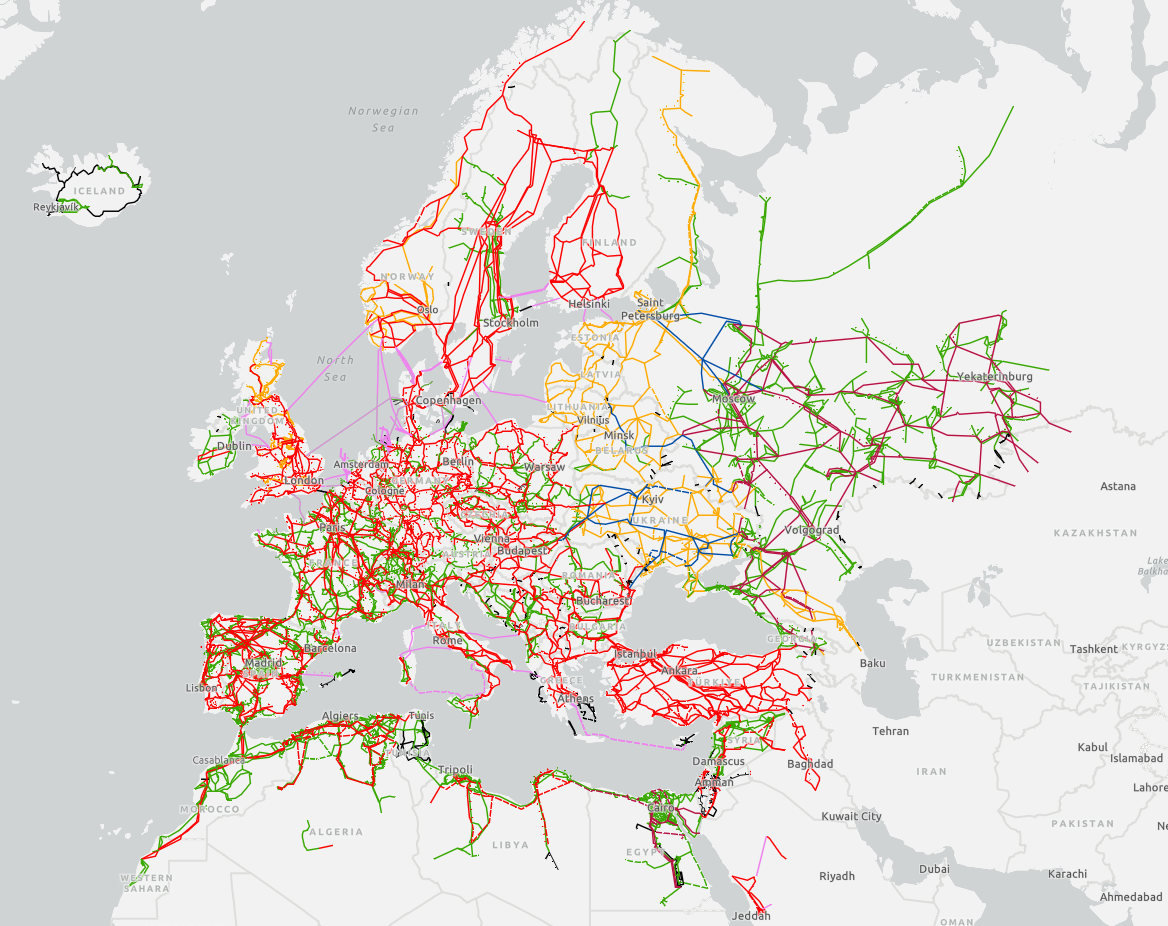
\includegraphics[width=0.68\textwidth]{chapter5pics/hvdcMap.png}
                \caption{Grid map of Europe, with HVDC links in purple.}
                \label{fig:hvdcMap}
            \end{figure}
        \end{column}
    \end{columns}
\end{frame}


% \subsection{Objectives}
\begin{frame}{Objectives}
    \begin{columns}
        % Left column with the image of GridCal
        \begin{column}{0.6\textwidth}
            \begin{figure}[H]
                \centering
                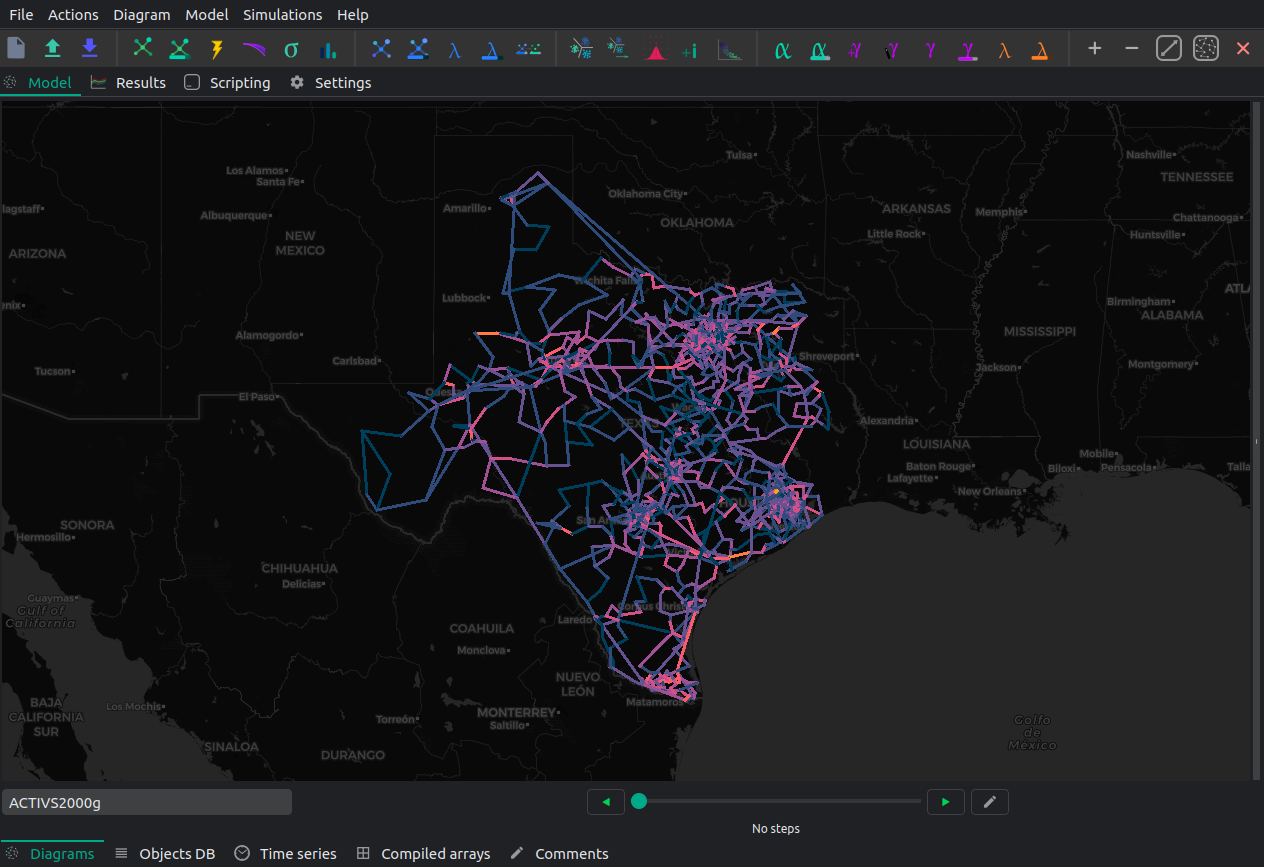
\includegraphics[width=0.95\textwidth]{chapter5pics/gridcalUI.png}
                \caption{GridCal interface used for power flow analysis in Spain.}
                \label{fig:gridcal_interface}
            \end{figure}
        \end{column}
        
        % Right column with the bullet points
        \begin{column}{0.4\textwidth}
            \begin{itemize}
                \item Integrate both AC and DC systems into a unified framework.
                \item Address the convergence issues found in current methods.
                \item Model complex components like converters and controllable transformers.
                \item Implement the method and test its scalability.
            \end{itemize}
        \end{column}
    \end{columns}
\end{frame}


% Include the comparison table after the Generalized Power Flow slide
\begin{frame}{Comparison of features}
    We present a generalised approach to the power flow problem, much more flexible than conventional methods.
    
    \begin{table}[htbp]
    \centering
    \begin{tabular}{|l|c|c|c|}
    \hline
    \textbf{Feature} & \textbf{Traditional} & \textbf{Classical} & \textbf{Generalised} \\ \hline
    Handles AC systems & \(\checkmark\) & \(\checkmark\) & \(\checkmark\) \\ \hline
    Remote controls & \(\times\) & \(\times\) & \(\checkmark\) \\ \hline
    Control more than two magnitudes at a bus & \(\times\) & \(\checkmark\) & \(\checkmark\) \\ \hline
    Controlled branch magnitudes & \(\times\) & \(\checkmark\) & \(\checkmark\) \\ \hline
    Interconnected AC/DC grids & \(\times\) & \(\checkmark\) & \(\checkmark\) \\ \hline
    Flexible bus type definition & \(\times\) & \(\times\) & \(\checkmark\) \\ \hline
    \end{tabular}
    \caption{Comparison between traditional, classical, and generalised power flow.}
    \label{tab:generalisedPfFeatures}
    \end{table}
\end{frame}





